\documentclass{../indiv}
\graphicspath{{../../images/part2/ch1/}}
\setcounter{chapter}{0}

\begin{document}
	\chapter{寫出你的第一份 \LaTeX 文件 !}
	
	\section{Hello, World! in \LaTeX}
	首先,請大家先進入到Texmaker中新增一份文件(預設快速鍵:\Ctrl+\keystroke{N}),並在畫面中間的原始碼區輸入以下的範例:
	\begin{latexex2}{``Hello, World!" in \LaTeX}
\documentclass{article}
\begin{document}
	Hello World!
\end{document}\end{latexex2}
	輸入完成後存檔(預設快速鍵:\Ctrl + \keystroke{S}),接著就可按下上方工具列的「快速編譯」(預設快速鍵:\keystroke{F1}),讓Texmaker自動呼叫我們先前設定的編譯器。編譯完成後,右側的內建PDF檢視器就會顯示編譯後的PDF檔,我們就不用自己打開Acrobat Reader在那邊慢慢比對,而這也是使用Texmaker的一大好處。整個畫面大概看起來像這樣:
	
	\begin{figure}[H]
		\centering
		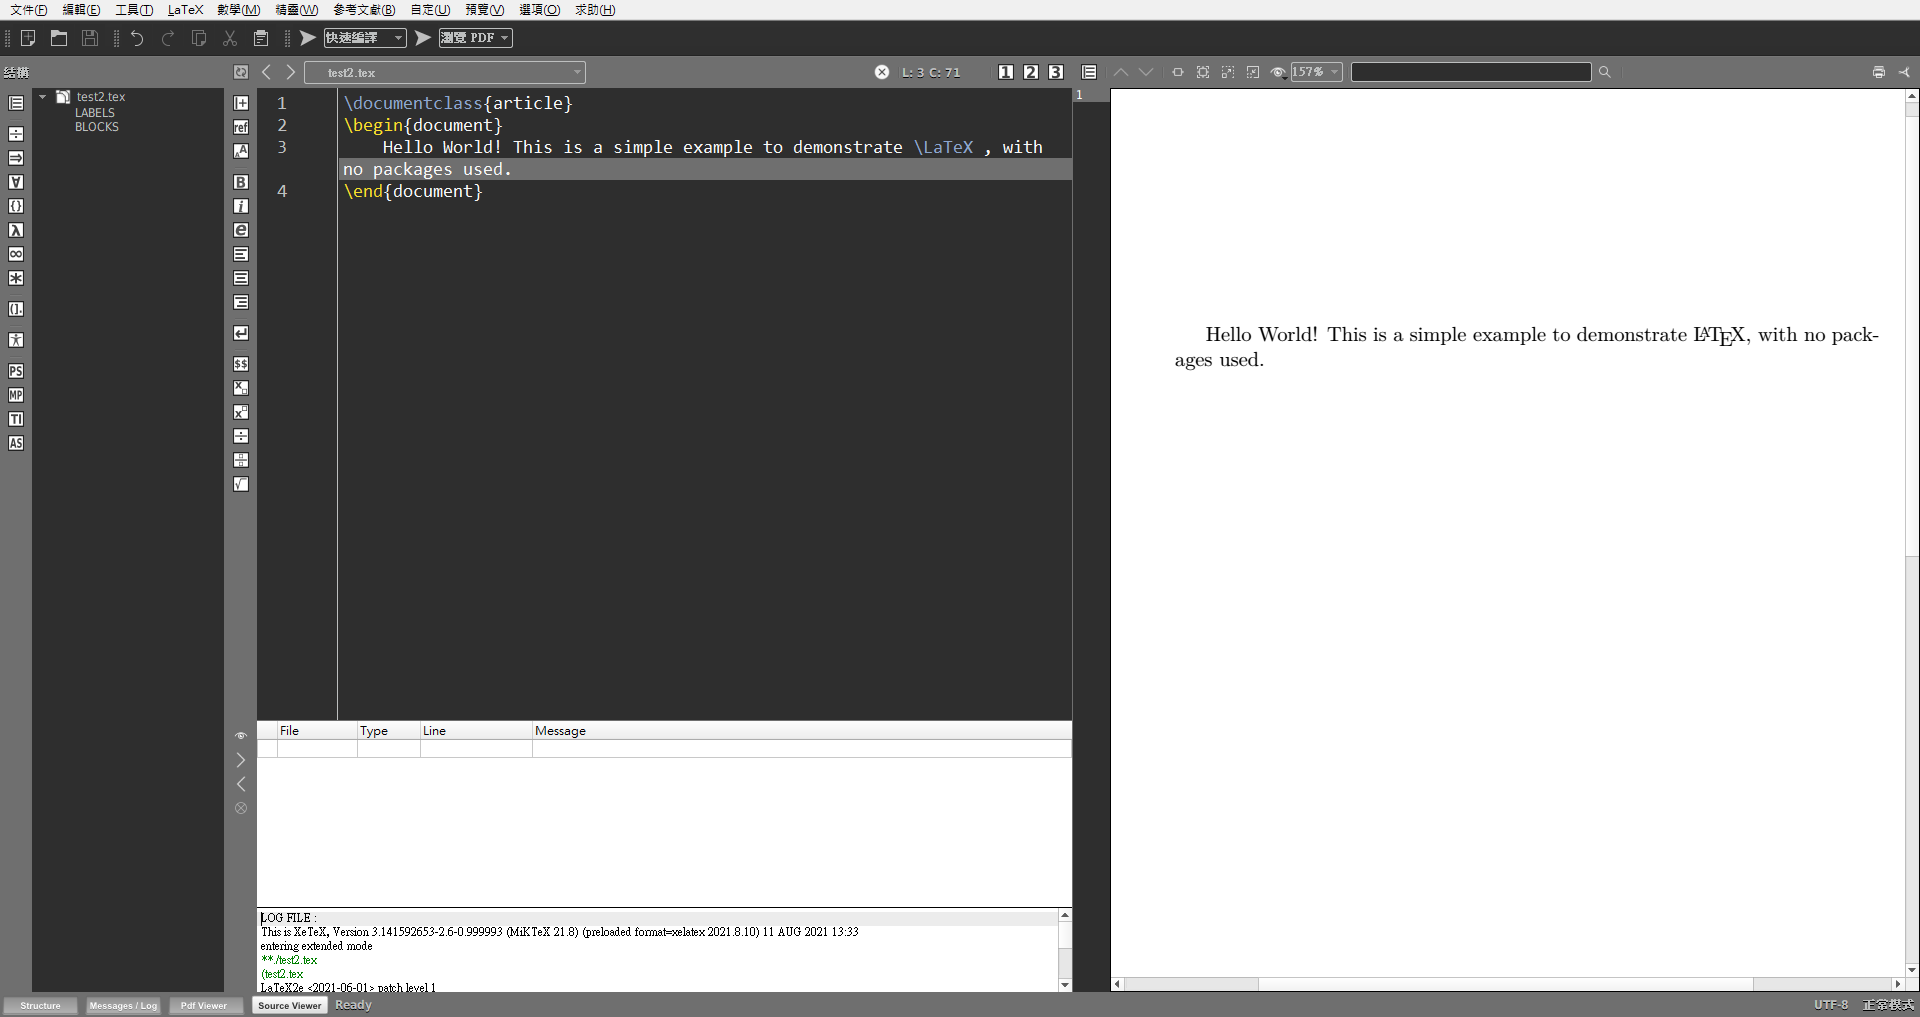
\includegraphics[width=0.8\linewidth]{texmaker-ex1.1-demo.png}
		\caption{完成快速編譯的Texmaker}
	\end{figure}
	




\end{document}